% Chapter 1

\chapter{绪论}
\section{研究背景与意义}
如今,机器人技术不断成熟,机器人在许多领域都发挥着越来越重要的作用。随着计算机视觉和深度学习的迅速发展,目标检测、目标跟踪等算法也越来越成熟,使得机器人的应用领域更加广泛。TX2、Manifold妙算等高性能机载电脑的出现,打破了机器人计算性能的壁垒,使得机器人可以完成更加复杂的任务。同时,随着视觉传感器、激光雷达、惯性测量单元等传感器的不断发展,以及算法的不断提出和改进,让机器人的自主定位、实时建图、自主导航等功能都变得可行、可靠。所有的这些进步,让机器人具有了更加强大的功能和更为广阔的应用,例如未知环境的探索,危险环境下的自主作业等。

同时,相较于传统的单个机器人的单独作业,多机器人的协作也显现出越来越大优势。单机器人系统实现简单,但所有的机器人都有其优势也有其弊端,因此单机器人系统的应用是受限的;而多机器人系统虽然较为复杂,但是有高性能机载电脑的支持,复杂算法已不是问题,多机器人系统通过机器人之间的协调合作可以进行优势互补,使得整个系统性能最大化,这是单机器人系统不具备的优势。目前,无人机和无人车是两种使用最为广泛、技术最为成熟的机器人,无人机具有高机动性和全局视觉,适用于侦察、检测等任务,但其续航能力弱,一般只能工作十几分钟,同时其载重量小,不适合挂载较多传感器和运输物体;无人车续航能力强,载重量大,可以执行抓取、运输等任务,但只具有局部视觉。当二者联合工作时,利用无人机广阔的环境感知能力可以为无人车提供全局的环境信息和导航信息,无人车具有的局部视觉可以使其更好地执行任务,二者的结合可以提高任务的完成度,因此无人机和无人车的联合工作在目标搜索方面具有很大的优势。

空地联合目标搜索也具有广泛的用途。在民用方面,可用于救援减灾、物流配送、城市垃圾清理等,既可以解放人力,又可以提高工作效率和质量;在军用方面,可以使用空地机器人联合执行侦察等任务,即保障士兵的安全,又保障任务的可靠完成;空地联合目标搜索也很容易扩展为其他应用,例如未知环境的快速探索和3D建图等。

\section{国内外研究现状}
目前在空地机器人联合目标搜索方面的研究在国际上较为深入,瑞士的苏黎世联邦理工学院(ETH Zurich)的Autonomous Systems Lab (ASL)和Robotic Systems Lab (RSL)共同实现了一种基于无人机和足式机器人的协同导航系统\upcite{r1},该系统先利用无人机扫描未知区域,通过SLAM (simultaneous localization and mapping)建立全局定位地图和半稠密点云地图,分别用于后续足式机器人的定位和导航。然后足式机器人利用视觉惯性里程计(VIO)和全局定位地图进行自身的定位,同时利用激光雷达的点云数据更新全局点云地图,并利用路径规划算法生成导航路径,指引足式机器人前往设置的目标处。该系统最大的两个优点是不需要外部的定位信息,例如GPS信号,也不需要无人机与地面机器人的相对位置信息,即无需无人机跟随地面机器人,因为该系统拥有全局定位地图,因此该系统的应用范围较广。但该系统对算法的精度要求非常高,因此算法较为复杂。

在国内,香港科技大学实现了一种复杂环境下的空地协同目标搜索系统\upcite{r2},该系统利用ArUco 标记作为搜索目标,以无人车的初始位置为坐标原点,无人车初始朝向为$x$轴,建立全局坐标系。该系统首先利用无人机扫描周围环境,进行目标检测和目标在全局坐标系下的定位。扫描结束后无人机将目标位置信息发送给无人车,然后开始跟随无人车,同时无人车启动。无人车行使过程中,无人机和无人机分别利用传感器测量自身的运动速度,同时无人机利用单目相机检测无人车和目标,一旦检测到无人机或目标,就通过PnP算法计算无人机与无人车或无人机与目标的相对位置信息,然后利用速度信息和相对位置信息通过EKF (Extended Kalman Filter)估计无人机和无人车的全局坐标,实现无人机与无人车的定位。同时利用激光雷达的点云数据和路径规划算法进行无人车的动态避障和导航。该算法也不需要GPS等外部定位信息,因此可以在室内、隧道等弱GPS或无GPS信号的环境下工作。但该系统要求无人机跟随无人车,同时只使用EKF实现无人机和无人车的定位会有累积误差。

此外,也有一些利用GPS信号进行定位的系统\upcite{r3,r4}。同时在空地联合环境探索方面国内外也有深入研究\upcite{r5,r6,r7,r8,r9},其方案也可以借鉴和参考。

\section{研究内容与结构安排}
参考国内外研究现状,本设计选择使用基准标记作为搜索目标,以实现目标的简单、快速检测和定位,同时利用GPS实现无人机与目标的定位,本项目的系统整体框架如图~\ref{fig:1-1}所示。

\begin{figure}[htb]
	\centering
	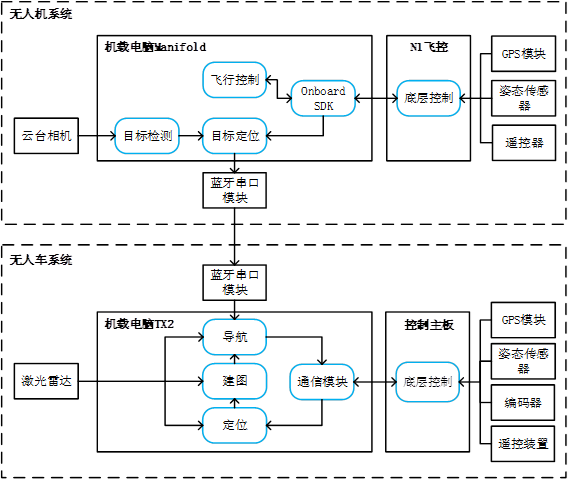
\includegraphics[width=\linewidth]{figures/1-1.png}
	\caption{系统整体框架}
	\label{fig:1-1}
\end{figure}

为了实现图~\ref{fig:1-1}所示的基于无人机-车的空地联合目标搜索系统,本项目主要研究了以下内容:

\begin{enumerate}[label=(\arabic*)] 
	\item 基准标记的检测与定位算法;
	\item 无人机的自主飞行;
	\item 无人车的运动控制,以及自主定位、建图和导航。
\end{enumerate}

本文结构安排如下:

第一章为绪论。主要介绍了基于无人机-车的空地联合目标搜索的研究背景与意义,国内外研究现状,以及本文的研究内容与结构安排。

第二章是无人机系统。首先介绍了无人机系统的硬件模块。接着详细介绍了AprilTag、ChromaTag和ArUco三种基准标记及其检测算法。然后分析了相机的成像模型,介绍了PnP算法和目标GPS坐标计算方法。最后介绍了无人机系统的软件设计。

第三章是无人车系统。首先介绍了无人车系统的硬件模块,然后详细介绍了无人车自主定位、SLAM建图和自主导航的实现方法,最后介绍了无人车系统的软件设计。

第四章是系统测试与结果分析。分别做了无人机系统的目标检测测试、目标定位测试和自主飞行测试,无人车系统的自主定位测试、SLAM建图测试和自主导航测试,以及系统整体测试,并进行了结果分析。

第五章是总结与展望。对目前完成的工作进行了总结,并分析了系统的不足以及尚未解决的问题,并对后续的改进和完善进行了展望。

\section{本章小结}
本章为全文绪论,首先介绍了基于无人机-车的空地联合目标搜索的研究背景与意义,然后分析了近年来国内外研究现状,大体介绍了几种系统设计方案,最后对论文的研究内容与结构安排做了简要描述。

